% !TEX encoding = UTF-8
% !TEX TS-program = pdflatex
% !TEX root = ../tesi.tex
% !TEX spellcheck = it-IT

%**************************************************************
\chapter{I template}\label{cap:template}
In questo capitolo viene descritto il lavoro svolto nella prima parte del progetto, che consiste nella realizzazione dei template, nel spiegare come sono stati resi responsive ed in fine come sia stato possibile inserire \textit{plug-in} JQuery al loro interno.\\
Viene anche trattato l'argomento relativo al loro caricamento all'interno della pagina HTML e la gestione delle librerie.
%**************************************************************
\section{Utilizzo di Ractive.js}
In questa sezione viene descritta più in dettaglio la libreria scelta per svolgere il progetto.
\subsection{L'oggetto Ractive}
Per iniziare ad usare Ractive bisogna innanzitutto creare un istanza dell'oggetto Ractive e passarle le opzioni desiderate tra quelle offerte dalla libreria.\\
Una volta creato l'oggetto questo si occuperà di creare e popolare il proprio registro dati e di creare in memoria una rappresentazione virtuale del template.\\
\begin{lstlisting}[language=JavaScript, caption=Creazione di un oggetto Ractive.]
var ractive = new Ractive({
	el: '#container', // id dell'elemento target nella pagina
	template: '<p>{{greeting}}, {{recipient}}!</p>', // esempio di template
	data: { greeting: 'Hello', recipient: 'world' } // oggetto JavaScript contenente i dati
});
\end{lstlisting}

\newpage

\subsection{Le opzioni principali}
La libreria fornisce un insieme consistente di opzioni che possono essere inizializzate alla creazione dell'oggetto Ractive.\\
Queste si dividono in sei categorie che sono le seguenti:
\begin{itemize}
	\item data;
	\item templating;
	\item transitions;
	\item binding;
	\item parse;
	\item lifecycle event.
\end{itemize}

Tutte queste opzioni opportunamente inizializzate vanno a definire le proprietà ed il comportamento del template nel suo intero ciclo di vita.\\
Le opzioni principali sono:
\begin{itemize}
	\item \textbf{el}: identifica l'elemento target all'interno del browser DOM dove verrà renderizzato il template;
	\item \textbf{template}: rappresenta il template da renderizzare;
	\item \textbf{data}: rappresenta i dati che dovranno essere interpolati con il template;
	\item \textbf{compute}: oggetto che può contenere espressioni o funzioni che verranno ricalcolate al variare del data model;
\end{itemize}

\subsection{Il two-way data biding}
La libreria fornisce la funzionalità di one-way-binding tra i dati contenuti nel data registry e il virtual DOM, cioè al variare del model il virtual DOM e di conseguenza anche la sua rappresentazione nel browser vengono modificate.\\
Oltre a questo tipo di legame, la libreria offre, per elementi di input , il two-way-binding, che permette di modificare il model al variare dei dati nella view e viceversa.
\begin{figure}[htp]
	\centering
	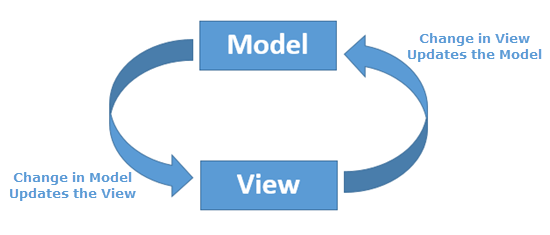
\includegraphics[width=\textwidth/2]{../immagini/twoWayBinding}
	\caption{Rappresentazione two way data binding.}
\end{figure}
\subsection{Gli eventi}
La libreria Ractive implementa il pattern architetturale  \textit{publish/subscribe}, che permette di rispondere o innescare particolari eventi, che attualmente vengono gestiti su due livelli.\\
Il primo è un interazione a basso livello con gli eventi del DOM che viene specificata tramite \textit{directives} del template che specificano anche  come l'evento deve essere gestito, tramite \textit{proxy event} o chiamate a metodi.\\
Il secondo è gestito dalle API \textit{publish/subscribe} e dal sistema di eventi all'interno di Ractive e tra i componenti.\\
I \textit{proxy events} collegano gli eventi del DOM con gli eventi di Ractive, mentre le chiamate a metodi direttamente sull'istanza ractive non utilizzano l'infrastruttura \textit{publish/subscribe}.
\subsection{Il virtual DOM}
Ractive utilizza un sistema differente dagli altri per tracciare le modifiche, ricorrendo al cosiddetto Virtual DOM, ossia a una rappresentazione virtuale della struttura del template immagazzinata in memoria e del tutto simile al DOM originale, del quale può essere vista come una astrazione.\\
Nel momento in cui si verifica un evento ed è necessario reagire ad esso modificando gli elementi della pagina, Ractive applica prima tali interventi al Virtual DOM.\\
Attraverso l’analisi delle differenze tra lo stato del Virtual DOM precedente al verificarsi dell’evento e quello nuovo ottenuto dall’applicazione delle modifiche, Ractive determina i cambiamenti effettivi da apportare al DOM vero e proprio.\\
Il calcolo delle differenze tra i due stati del DOM virtuale è estremamente veloce, e grazie a esso si limitano al minimo indispensabile gli interventi sul DOM reale, tendenzialmente più lento, garantendo quindi ottime performance.

\subsection{Plug-in di terze parti}\label{sec:packager}
I \textit{plug-in} permettono di aumentare le funzionalità offerte dalla libreria Ractive.\\
Agli sviluppatori è data la possibilità di creare i propri \textit{plug-in} o di scegliere quelli più adatti alle proprie esigenze da una lista presente sul sito di Ractive.js.\\
Durante lo sviluppo del progetto sono stati utilizzati i \textit{plug-in} \href{https://github.com/ractivejs/ractive-events-tap}{ractive-events-tap}, per gestire il click/tap sui dispositivi mobili , e \href{https://github.com/ractivejs/ractive-load}{ractive-load}, per il caricamento tramite protocollo \textit{http} dei template.   

\section{Sviluppo dei template}
La creazione dei template, per il progetto, non presentava nessuna restrizione né per la forma né per i contenuti, quindi la decisione di quali template sviluppare era a discrezione del programmatore.\\
L'unica richiesta, per questa fase del progetto, è stata quella di avere template sia HTML che SVG.\\
\subsection{Struttura dei template}
I template HTML sono strutturati come una pagina web, cioè sono formati dal codice HTML per quanto riguarda i contenuti, il codice CSS per la loro rappresentazione grafica e JavaScript per definire il loro comportamento.\\
Il codice HTML rappresentante il template deve essere arricchito tramite la sintassi \textit{mustache} contenente le variabili, le espressioni e tutti gli elementi utili al funzionamento del template.\\
Inoltre possono essere presenti le direttive necessarie nel caso il template presenti la possibilità di interazione con esso.\\
Il comportamento del template viene sviluppato tramite gli strumenti offerti dalla libreria Ractive.\\
La libreria permette di creare un singolo file che contiene al suo interno l'intero template cioè HTML+mustache, CSS e Javascript.\\
Questo risulta molto vantaggioso per diminuire la quantità di file e migliorare l'organizzazione dei vari template.\\
Ogni template dovrà inoltre avere un file con estensione \textit{.json} contenente i dati da visualizzare ed eventuali immagini o librerie necessarie per il suo corretto funzionamento.\\
I vari template sono stati suddivisi in cartelle nel seguente modo:
\begin{figure}[htp]
	\centering
	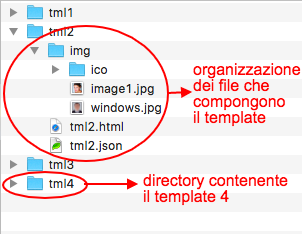
\includegraphics[width=\textwidth/2]{../immagini/fileSistemTemplate}
	\caption{Organizzazione dei template nel file system.}
\end{figure}

\newpage

\subsection{Prototipo di template}
Di seguito viene riportato una parte del codice utilizzato per la creazione di un template HTML.\\

\begin{lstlisting}[language=HTML, caption= Esempio di template.]
<div id="tml1" style="background-color: {{bgColor}}; color: {{textColor}};">
	<img class="image" src= {{ img ? img : 'templates/tml1/img/no-image.png'}}>
	<div class="prod-data">
		<h2 class="center">{{nome}}</h2>
		prezzo: <strong>{{prezzoCent}} euro</strong>
		<p class={{ quantita ? 'disponibile' : 'non-disponibile'}}>Disponibilità: 
		{{#if quantita}}
			<strong>disponibili {{quantita}}</strong>
		{{else}}
			<strong>Non disponibile</strong>
		{{/if}}
		</p>
		<h3>Descrizione:</h3>
		<p class="desc">{{descrizione}}</p>
	</div>
</div>

<!-- stili -->
<style>
	<!-- parte relativa alle regole CSS -->
	...
</style>

<script>
	<!-- parte relativa al comportamento del template -->
	component.exports = {
		computed: {
			prezzoCent: function(){
				return this.get('prezzo').toFixed(2);
			}
		}
		...
	}
</script>
\end{lstlisting}

Come si può notare il file è suddiviso in tre sezioni.\\
La prima contiene il codice HTML con l'aggiunta di variabili ed espressioni inserite tramite mustache.

\begin{lstlisting}[language=HTML, caption= Espressione con mustache.]
<p class={{ quantita ? 'disponibile' : 'non-disponibile'}} >
\end{lstlisting}

Nell'esempio sopra riportato il codice permette di modificare l'attributo "classe" del tag \textit{p} in base al valore della variabile \textit{quantita}.\\
La porzione di codice seguente rappresenta una condizione \textit{if} che visualizza nel template la stringa \textit{"disponibili: numero prodotti"} se \textit{quantita} è maggiore di 0 e \textit{"non disponibile"} altrimenti.

\newpage

\begin{lstlisting}[language=HTML, caption=Condizione if-else con mustache.]
	{{#if quantita}}
		<strong>disponibili {{quantita}}</strong>
	{{else}}
		<strong>Non disponibile</strong>
	{{/if}}
\end{lstlisting}

Il file contiene anche l'implementazione dell'opzione \textit{computed} fornita dalla libreria Ractive.js che verrà utilizzata durante la creazione dell'oggetto Ractive.\\
Tramite il metodo \textit{export} di component è possibile definire la logica del template utilizzando le opzioni e i metodi forniti dalla libreria Ractive.js.\\
In questo caso viene indicato che ogni volta che il prezzo subisce modifiche questo deve essere convertito in una stringa e rappresentato con due decimali.

\begin{lstlisting}[language=JavaScript, caption=Implementazione ed esportazione opzione computed.]
component.exports = {
	computed: {
		prezzoCent: function(){
			return this.get('prezzo').toFixed(2);
		}
	}
	...
}
\end{lstlisting}

Al template viene fornito un oggetto JSON contenente dei dati di default, utilizzati per ottenere una rappresentazione del template completa.\\
Questi dati sono contenuti in un file con estensione \textit{.json} presente all'interno della directory del template.\\
L'oggetto JSON è definito come segue.

\begin{lstlisting}[language=JavaScript, caption=Rappresentazione dell'oggetto JSON.]
{
	"bgColor":"#ededed",
	"textColor":"#000000",
	"nome": "Cuffie rosse WiFi",
	"img": "templates/tml1/img/cuffie.jpg",
	"prezzo": 200,
	"quantita": 6,
	"descrizione": " ... "
}
\end{lstlisting}

\newpage

In seguito vengono proposte due immagini del template descritto in precedenza dopo il rendering da parte della libreria Ractive.js.\\
Queste immagini fanno vedere come cambia la rappresentazione del template quando la variabile \textit{quantita} è maggiore di 0 e quando è uguale a 0.
\begin{figure}[htp]
	\centering
	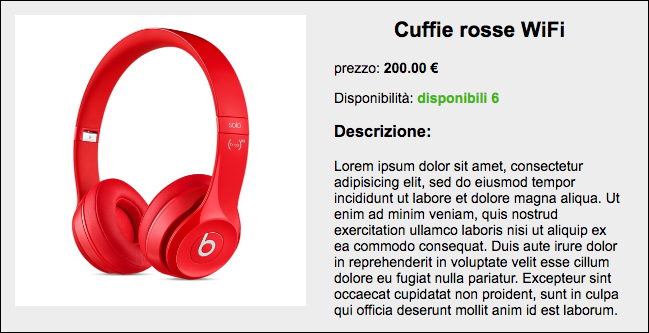
\includegraphics[scale=0.4]{../immagini/screenshot_tml1_1}
	\caption{Rappresentazione del template con \textit{quantità} maggiore di 0.}
	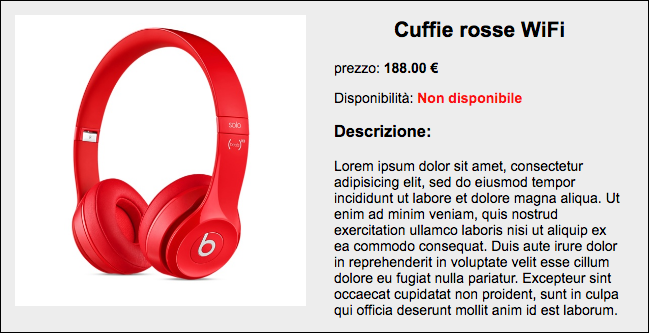
\includegraphics[scale=0.4]{../immagini/screenshot_tml1_2}
	\caption{Rappresentazione del template con \textit{quantità} uguale a 0.}
\end{figure}

Nel caso in cui il template utilizzi SVG, la struttura del template è la stessa, con l'unica differenza che la sintassi mustache viene aggiunta al codice SVG.
\section{Rendere il template responsive}
Uno dei requisiti richiesti per quanto riguarda lo sviluppo dei template è quello di renderli \textit{responsive}, in modo che sia possibile visualizzarli su dispositivi desktop e mobile.\\
La soluzione individuata per soddisfare questo requisito è stata quella di inserire delle \textit{media-query} all'interno del CSS del template, definendo le regole per la corretta rappresentazione a diverse risoluzioni.\\
La pagina che andrà ad ospitare i template dovrà contenere il meta-tag \textit{viewport} per garantire la corretta visualizzazione.\\
Utilizzando questo metodo si riesce a mantenere il CSS all'interno del file che contiene il template, senza ricorrere ad uno o più file esterni contenenti le regole relative a vari dispositivi.\\
\newpage
Di seguito viene proposto un esempio di media query.
\begin{lstlisting}[language=JavaScript, caption=Esempio di media query nel CSS del template.]
@media only screen and (min-width: 320px) and (max-width: 639px){

	.image{
		width: 90%;
		...
	}
	
	.prod-data{
		float: none;
		..
	}

	...
}
\end{lstlisting}

\section{Inserimento plug-in jQuery nei template}
Oltre a rendere i template responsive, un'altra richiesta da soddisfare durante questa fase del progetto consisteva nello studiare la possibilità di sviluppare template che contenessero plug-in JQuery.\\
L'utilizzo di plug-in JQuery implica:
\begin{itemize}
	\item il caricamento della libreria del plug-in;
	\item la stesura del codice HTML seguendo le regole fornite dallo sviluppatore della libreria;
	\item la stesura di uno script JavaScript che va a richiamare le funzionalità desiderate tra quelle offerte dal plug-in.
\end{itemize}
Questo particolare script deve essere eseguito in seguito al caricamento del template all'interno della pagina.\\
La soluzione individuata per avere template che contengano plag-in JQuery consiste nell'inserire lo script per il funzionamento del plug-in come implementazione dell'opzione \textit{oncomplete} dell'oggetto Ractive.\\
L'opzione \textit{oncomplete} fa parte dei \textit{lifecycle events} di Ractive e viene richiamata nel momento in cui il template è stato completamente renderizzato.\\
Questa soluzione oltre a permettere l'inserimento dello script all'interno del file del template, assicura che la sua esecuzione avvenga in maniera corretta.\\
In seguito viene riportato un esempio di implementazione dell'opzione \textit{oncomplete} per l'utilizzo di un plug-in jQuery.
\begin{lstlisting}[language=JavaScript, caption= Implementazione dell'opzione \textit{oncomplete}]
<script>
	component.exports = {
		oncomplete: function() {
			jQuery(this.find('#img1')).actuate('wobble');
			jQuery(this.find('#img2')).actuate('pulse');
		}
	}
</script>
\end{lstlisting}
\section{Caricamento dei template nelle pagine HTML}

